\chapter{Implementing \enquote{lox}}

\vspace{-8mm}
\begin{figure}[h]
  \centering
  
\includegraphics[width=.2\textwidth]{svg2pdf/logo-lox-preliminary}
  \caption{Preliminary logo of \codebox{lox}.}
\end{figure}
\vspace{8mm}

This chapter discusses the major design decisions and notable implementation details behind \code{lox}.
In the end, a short overview over all features offered by the library is presented.
As already mentioned in the introduction, \code{lox} is licensed as MIT/Apache-2.0 and is developed here: \url{https://github.com/LukasKalbertodt/lox}.

The library consists of a single crate (one minor exception is explained later) which is very common for medium-sized Rust libraries.
As \code{lox} contains a variety of features, it is likely that some users do not need all of them.
To avoid compiling parts of the library that are unused, \code{lox} uses \emph{Cargo features} to let the user disable those parts individually.
For example, if a user does not read from or write to files, the IO module can be disabled completely and thus will not be compiled or linked.

To maintain a high code quality, various automated tests and checks are used.
These are further explained in the respective sections of this chapter.
All of these tests are automatically executed on a \emph{continuous integration} (CI) server whenever commits are pushed to the repository or a \emph{pull request} is created.
The CI also builds the documentation and makes sure that no compiler warnings are emitted.


\vfill
\begin{center}
  \begin{minipage}{.9\textwidth}
    \small
    As an aside:
    the term \enquote{lox} is often used as an abbreviation for \emph{\textbf{l}iquid \textbf{ox}ygen}, a pale-blue liquid usually obtained by cooling elemental oxygen below its boiling point of 90.188\,K.
    This substance is used in many areas, playing a particularly important role in the aerospace industry where it is commonly used as a cryogenic oxidizer in rockets.
    Since rust (the chemical compound\footnotemark) is a product of an oxidation reaction and rockets are usually fast, using \enquote{lox} as name for this library seemed fitting.
    However, the name was mainly chosen because it is short and pronounceable.
  \end{minipage}
\footnotetext{The programming language \emph{Rust} is not even named after the chemical compound, but after the \enquote{Rust} family of fungi. Source: \url{https://www.reddit.com/r/rust/comments/27jvdt/}}
\end{center}


\newpage
\section{Basic Memory Layout Considerations}
\label{chap:memory-layout}

\subsubsection*{Element Reference}

In many situations, it is necessary to refer to a specific element in the mesh (for example, to delete a specific face or to query the neighbors of a specific vertex).
There are mainly two ways to realize an \emph{element reference}: pointers or IDs/indices.
As discussed in chapter~2, it is desirable to use growing arrays to store mesh data, making pointers impossible (or at least very difficult) to use as element references.
As a consequence, \code{lox} uses the index of an element in its array to refer to that element.
(Also refer to \cite{sieger2011design} for a discussion about array vs. linked lists and indices vs. pointers.)

Using simple integers as element references in the library's API is not a good idea, however, since it is very easy to use an integer referring to one element kind (e.\,g. a vertex) in a context where a reference to another element kind (e.\,g. a face) is expected.
To avoid this confusion, multiple distinct types are introduced: \code{VertexHandle}, \code{EdgeHandle} and \code{FaceHandle}.
All of those types consist of a single integer field (called the \emph{handle ID}), making them behave exactly like an integer on machine level -- thus having no runtime overhead.
If one is used in the place of another, a compiler \enquote{type mismatch} error is printed, pointing out the bug immediately.
Additionally, a \code{Handle} trait is defined to abstract over all handle types.

Another benefit of dedicated handle types is that the internal integer type can be changed easily (without changing it across the whole codebase).
The default integer type in \code{lox} is a \code{u32} which is sufficient for most meshes in practice.
However, large meshes with more than $2^{32}$ elements require a wider integer type.
With the already mentioned Cargo features, it is possible to configure \code{lox} to used \code{u64} integers in handles, which is sufficient for all meshes in the foreseeable future.

\vspace{2cm}
\subsubsection*{Deleting Elements in a Growable Array}

A simple growing array cannot replace a linked list in all situations, since the latter allows to remove elements anywhere in the list in $\mathcal O(1)$ whereas the former only supports removing elements from the end.
Being able to remove arbitrary elements from a mesh required in many situations, so mesh data structures are expected to support it.

There are two possibilities to remove an element at any position inside an array: (a) shift all elements right of the deleted elements one to the left, and (b) store a \code{deleted} flag for each element which is set to \code{true} once an element is deleted.
Solution (a) has a complexity of $\mathcal O(n)$ per remove-operation, making it too slow for most applications.
However, the real problem is that shifting elements invalidates their indices which are used as element reference.
As a consequence, solution (b) has to be used.

\newpage
A problem of the \code{deleted}-flag approach is that elements are not actually deleted but linger in memory, potentially until the whole data structure is freed.
To avoid wasting a lot of memory, programmers should avoid repeatedly adding and removing a large number of elements.
Additionally, the mesh data structure can offer the programmer a way to trigger an internal garbage collection which actually removes deleted elements by reordering the elements in the array.

There are different ways to implement the \code{deleted} flag.
The easiest and most obvious solution in Rust would be to use \code{Vec<Option<T>>} instead of \code{Vec<T>}.
In practice, storing many \code{Option<T>} instances is only a good idea if \code{Option<T>} can use \emph{null value optimization}.
This is usually not the case in the context of mesh data structures, meaning that \code{Option<T>} is notably larger than \code{T}.
Specifically, it is \code{align_of::<T>()} larger, which for structs storing \code{u32} indices is usually 4 bytes.

\begin{figure}[t]
  \centering
  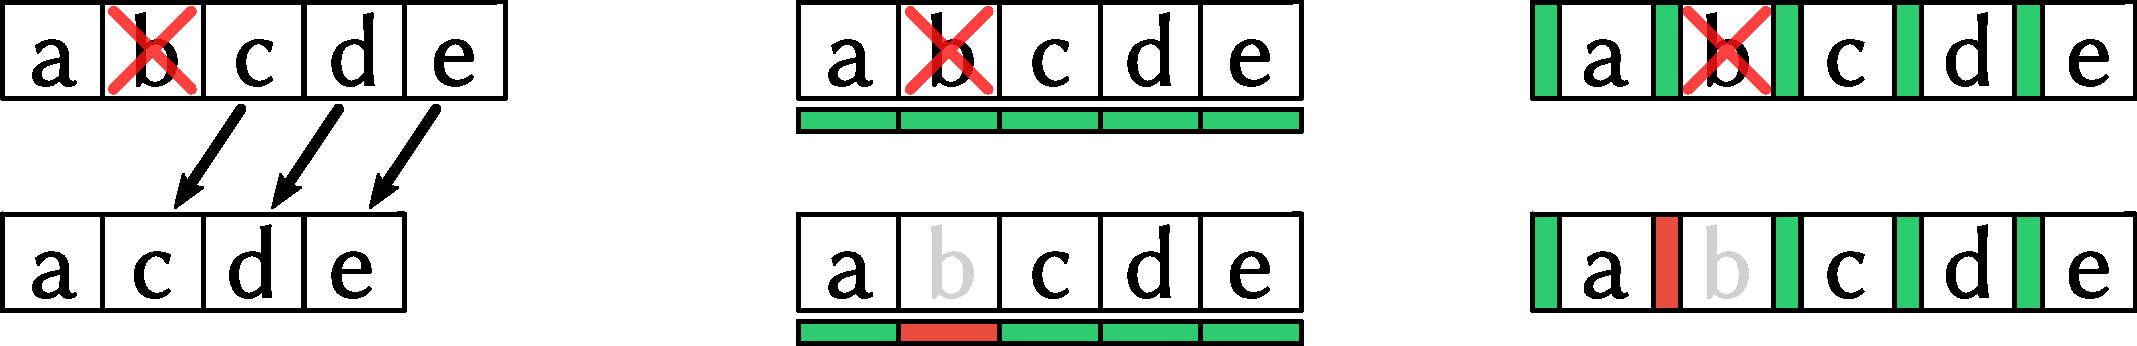
\includegraphics[width=.9\textwidth]{svg2pdf/stable-vec}
  \caption{Different ways to delete an element from a growable array: shifting elements (left), storing a \codebox{deleted} flag as a separate bit-vector (center) and storing a \codebox{deleted} flag next to the elements (right).}
  \vspace{5mm}
\end{figure}

A popular alternative way to store \code{deleted} flags is using a bit-vector, a densely packed array of bits (storing 8 bits per byte).
It has the disadvantage of requiring a separate allocation which slightly increases the reallocation cost and could potentially double the number of cache misses per element access.
However, this is usually out-weight by the benefits:
the dense packing means that no memory is wasted and that many of these flags fit into the cache at once.
For example, a standard-sized L1 cache with 256~KB of storage can fit over 2~million bits, a 64~byte cache line can fit 512 bits.

It is also possible to use special \emph{sentinel values} to mark an element as deleted (this is the general case of null-value optimization, where the sentinel value is 0) or to interleave the bits with the actual values in blocks to avoid an additional allocation.
A proper analysis of these different storage methods would be appropriate, but was outside the scope of this thesis.
In a quick comparison of the \code{Vec<Option<T>>} and bit-vector versions, no large difference in performance was found.
As a consequence and for memory efficiency, the bit-vector implementation was chosen for \code{lox}.
This choice is not final, however, and the implementation could easily be replaced by another one.

The logic for growable arrays that allow deletions is implemented completely independently of \code{lox} in a library called \code{stable-vec}\footnote{\url{https://crates.io/crates/stable-vec}}.
This library is technically also not part of this thesis.





\newpage
\subsubsection*{Property Maps}

As mentioned in chapter 2, it is often necessary to associated arbitrary data with specific mesh elements.
This data is called \enquote{property} in this thesis; vertex normals are a \enquote{vertex property}, for example.
While some properties live as long as the mesh itself (e.\,g. vertex positions or face colors),  others are temporary values that only live for the duration of one algorithm (e.\,g. a Boolean \code{visited} flag).
These temporary properties should not be kept in memory longer than necessary, meaning that they cannot be stored together with the actual elements.
Instead, \code{lox} uses external maps (mapping from element to property), called \emph{property maps}.

These maps can be implemented in a variety of ways, including:

\begin{itemize}
\item A growing array using the handle ID as index (this works because it is already used as an array index in the main mesh).
\item A hash map using the handle ID as key.
\item A list of \code{(handle, value)} pairs.
\end{itemize}

In most situations, the growing array is the best choice as it is very memory efficient and accessing values is very cheap.
However, in a few situations it is necessary to associate values with only a couple of elements.
Using a growing array for that purpose is not a good idea, since the length of the array does not depend on the number of values but on the highest handle ID.
So on average, a growing array would waste a lot of memory, making other implementations a viable choice.

Just like with the mesh data structure, it does not make sense to decide on one specific implementation of external maps.
Instead, all implementations are offered by \code{lox} and abstracted over via traits.
That way, the most fitting implementation can be chosen in every situation.
The corresponding types are currently called \code{VecMap} (growable array), \code{HashMap} and \code{TinyMap} (list of tuples).
The abstraction is realized with three traits to make it as flexible as possible:

\begin{description}
  \item [\codebox{PropMap}] This trait only requires a single method to be implemented.
  Its signature is \code{fn get(&self, handle: H) -> Option<Value>} where \code{H} is the handle type parameter (this is a simplified version of the actual signature, which is explained in chapter~6).
  Returning \code{None} means that no value is associated with the given handle/element.
  This trait represents a simple map from handle to optional value.
  \item [\codebox{PropStore}] Like \code{PropMap}, but can additionally iterate over all handles and values.
  \item [\codebox{PropStoreMut}] Like \code{PropStore}, but can additionally change, insert and remove values.
\end{description}

The three data structures mentioned above (growing array, hash map, list of pairs) implement all three traits.
The reason for using three traits instead of a single one was to allow for more exotic type to be used with that interface.
The following types are provided by \code{lox} and implement \code{PropMap}, but not the other traits:

\newpage
\begin{itemize}
\item \code{EmptyMap}: contains no properties, always returns \code{None}.
\item \code{ConstMap}: stores a single value and returns that value for all elements/handles.
\item \code{FnMap}: stores a function object with the signature \code{(&self, H) -> Option<Value>} which is used to implement \code{PropMap}.
\end{itemize}

While these types might not seem particularly useful at first, they are immensely handy in some situations.
Of course, they can be replaced by simply preparing a growable array or hash map with the desired values.
This, however, costs memory and extra time.
Specifically, \code{FnMap} is very useful to generate properties without using memory.

As a motivating example, consider an algorithm that produces a float value for each face, thus returning \code{VecMap<FaceHandle, f32>}.
This float value needs to be visualized via colors, for example by simply mapping the float value to gray-scale colors.
With \code{FnMap} a face~$\rightarrow$~color mapping can be created easily without allocating any memory:

\begin{center}
  \begin{minipage}{.59\textwidth}
    \begin{rustcode}
      let face_values = algorithm(&mesh);
      let face_colors = FnMap(|fh| {
          face_values.get(fh).map(to_color)
      });
    \end{rustcode}
  \end{minipage}
\end{center}

\vfill
\subsubsection*{\enquote{Array of Structs} vs. \enquote{Struct of Arrays}}

Having property maps to store mesh properties externally brings up an interesting consideration: is it faster to use one property map per property kind or to use as few different maps as possible (e.\,g. by clustering different property kinds).
This problem is very similar to the \enquote{Array of Structs} (\emph{AoS}) vs. \enquote{Struct of Arrays} (\emph{SoA}) choice.
The two different layout strategies are visualized in figure~\ref{fig:mem-layout-visualization}.

Both layouts use almost the same amount of memory and do not differ in capabilities.
The only difference is in how they interact with CPU caches.
To find an answer to what strategy should be preferred, a number of different benchmarks were conducted.

\vspace{8mm}
\begin{figure}[b]
  \centering
  \newcommand{\pointerbox}{%
    \parbox{1.2cm}{%
      \tikz{%
        \draw (-3.2mm,-3.2mm) rectangle (3.2mm,3.2mm);
        \draw[line width=.4mm, {Circle[length=1.5mm,width=1.5mm]}-{Triangle[length=2.2mm,width=2.7mm]}](-0.75mm,0)--(1.2cm,0);
      }%
    }
    \hspace{2mm}
  }
  \renewcommand{\arraystretch}{1.1}
  \setlength{\dashlinedash}{.4mm}
  \setlength{\dashlinegap}{.4mm}

  \begin{subfigure}[b]{.55\textwidth}
    \centering
    \setlength{\tabcolsep}{0mm}
    \pointerbox
    \begin{tabular}{|C{6.2mm}:C{6.2mm}:C{6.2mm}|C{6.2mm}:C{6.2mm}:C{6.2mm}|C{6.2mm}:C{6.2mm}:C{6.2mm}|}\hline
      $a_0$ & $b_0$ & $c_0$ & $a_1$ & $b_1$ & $c_1$ & $a_2$ & $b_2$ & $c_2$ \\\hline
    \end{tabular}
    \vspace{7mm}
    \caption{Array of Structs.}
  \end{subfigure}%
  %
  \begin{subfigure}[b]{.35\textwidth}
    \centering
    \setlength{\tabcolsep}{0mm}
    \pointerbox
    \begin{tabular}{|C{6.2mm}|C{6.2mm}|C{6.2mm}|}\hline
      $a_0$ & $a_1$ & $a_2$ \\\hline
    \end{tabular}\\[-.5mm]
    \pointerbox
    \begin{tabular}{|C{6.2mm}|C{6.2mm}|C{6.2mm}|}\hline
      $b_0$ & $b_1$ & $b_2$ \\\hline
    \end{tabular}\\[-.5mm]
    \pointerbox
    \begin{tabular}{|C{6.2mm}|C{6.2mm}|C{6.2mm}|}\hline
      $c_0$ & $c_1$ & $c_2$ \\\hline
    \end{tabular}
    \caption{Struct of Arrays.}
  \end{subfigure}

  \renewcommand{\arraystretch}{1.0}

  \caption{The two different memory layouts (three items with three fields each).}
  \label{fig:mem-layout-visualization}
\end{figure}

\newpage
In these benchmarks, many items with a few random \code{u32} fields were stored in either one of the two memory layouts.
The time required to sum up all or some of these values was measured to get an idea of the respective speeds.
The different benchmarks attempted to cover the following parameter space:

\begin{itemize}
  \item \textbf{Memory layout}: AoS or SoA.
  \item \textbf{Traversal kind}: random or sequential.
  In the sequential benchmarks, a loop simply iterates sequentially over all indices starting from 0.
  The random benchmarks use the first field's \code{u32} value as next index to jump to.
  This was done to not include the generation of random numbers in the measured time.
  Notably, these \code{u32} values were already generated to be valid indices (i.\,e. smaller than the total number of items) and thus, the timed code does not need to perform any additional work on these values.
  \item \textbf{Total number of items}: all benchmarks were performed with 10,000, 100,000, 1,000,000 and 10,000,000 items.
  \item \textbf{Number of [used] fields per item}: 1:1, 2:1, 2:2, 4:1, 4:2, 4:4, 6:1, 6:3 and 6:6 were tested.
  The syntax X:Y means that each item has X many fields and Y many fields were included in the sum, the other fields were ignored.
\end{itemize}

\vfill

Getting reliable data from a benchmark is difficult because many factors need to be considered -- failing to pay attention to one of them could render the measured data useless.
To deal with the inherent noise, almost all benchmarks execute the code that needs to be measured many times and analyze all measured durations to obtain a useful point estimate (e.\,g. the mean).
Performing a benchmark that attempts to measure the effect of CPU caches is particularly challenging, because the cache state persists over multiple iterations of the same code.
That in turn means that repeated measurements are not independent from one another, making the measured data unusable or very hard to analyze.

One idea on how to tackle this problem is to simply flush all caches.
This is actually possible on most x86-64 CPUs with the \code{WBINVD} instruction, which first writes all cache contents back to main memory and then invalidates all CPU internal caches\footnote{There is also the \codebox{INVD} instruction which invalidates caches without writing them back, but it is highly unsafe as it globally destroys the consistency of memory operations, likely crashing or corrupting all programs currently running on the CPU (including the kernel).}.
As \code{WBINVD} is a privileged instruction, it can only be executed in ring 0 (the kernel mode).
But since benchmarks should not run in kernel mode, a special kernel module was loaded, allowing user-land programs to trigger execution of \code{WBINVD}.
The benchmarking code would use that trigger before each repetition of the benchmarked code.

Unfortunately, executing the instruction via the kernel module itself takes a significant amount of time (approximately 750\,µs on the benchmark machine).
Many of the benchmarks have a per-iteration time of less than that, making \code{WBINVD} a non-tolerable overhead.
Excluding the duration of cache invalidation from the total measured time is not easily possible either.
Since measuring short durations does not yield reliable data, multiple repetitions are measured together and not on their own.
Because of this massive overhead, \code{WBINVD} was dropped as possible solution.

\newpage
As an alternative, each repetition of the benchmark was performed on separate data.
Before executing the benchmarked code, a copy of the working data was prepared for each iteration, meaning that the cache state produced by one repetition does not affect other iterations.
As CPU caches have very complex behavior, the absence of cross-repetition cache effects cannot be completely guaranteed, but the probability of them occurring was reduced substantially.

The benchmark code and more details on the benchmark can be found in the repository of this thesis in the folder \code{benchmarks/memory-layout/}.
The benchmark uses the framework \emph{Criterion} \cite{criterion} which features a sophisticated statistical analysis of the raw measurements.
However, only the mean and standard deviation were used to produce the graph seen in this report.

The actual measurements was performed on a completely idle \textsf{Thinkpad T-460p}, containing an \textsf{Intel i7-6700\,HQ} and running \textsf{Ubuntu 18.04}.
The \textsf{Intel i7-6700\,HQ} has 6\,MiB of L3 cache, 1\,MiB of L2 cache and 256\,KiB of L1 cache.
The full benchmark ran for approximately three hours.
The results can be seen in figure~\ref{fig:memory-layout-bench} and are discussed on the page thereafter.

\begin{figure}[p]
  \centering
  \vspace{-7mm}
  \centerline{
    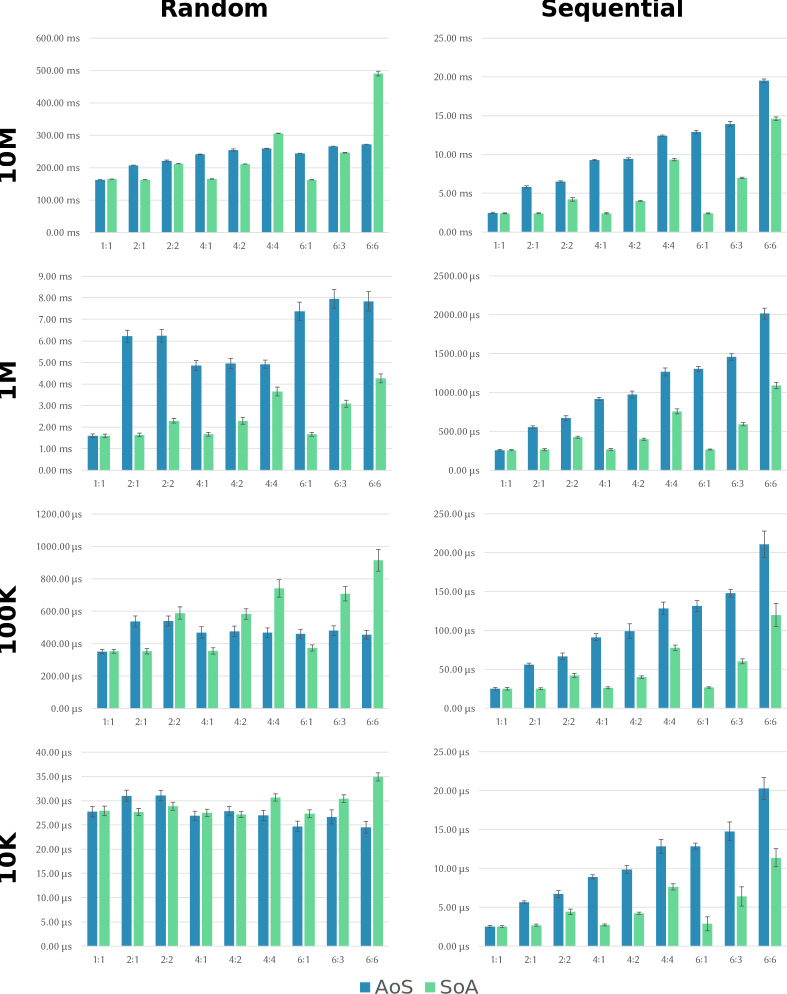
\includegraphics[width=1.18\textwidth]{svg2pdf/SOAvsAOS}
  }
  \caption{
    Results of the memory layout benchmark.
    The numbers on the far left show the total number of items.
    The label for each pair of bars encodes the number of fields: \textsf{X:Y} means that each item has \textsf{X} fields, \textsf{Y} of which are used.
    The height of the bars is the mean of all measurements, the error bar displays the standard deviation.
  }
  \label{fig:memory-layout-bench}
\end{figure}

\newpage

The results of the benchmark allow various interesting observations:

\begin{itemize}
  \item The type of traversal plays a massive role in performance: in the 10M items benchmarks, random traversal is approximately 50 to 70 times slower than the sequential traversal.
  The difference is a bit smaller for the benchmark with fewer items, but still substantially.
  This effect is very much expected.
  \item The durations for sequential traversal scale pretty closely with the number of items.
  This is to be expected, because in those benchmarks, any caching effects should be very small and all other operations should scale linearly.
  On the other hand, the durations for random traversal do \emph{not} scale linearly with number of items, due to non-linear cache effects.
  The difference between 1M and 10M items is particularly high.
  \item The durations of \textsf{1:1} benchmarks do not differ between memory layouts, which is expected: for one field, the memory layouts are the same.
  This is a confirmation that there are no unexpected differences in the benchmarks of different memory layouts.
  \item The duration for SoA benchmarks does not depend on the total number of fields, but just on the number of \emph{used} fields.
  For example, \textsf{1:1}, \textsf{2:1}, \textsf{4:1} and \textsf{6:1} take the same time.
  This makes sense because adding additional, unused fields does not affect which memory is accessed by the SoA benchmark.
  \item For random traversal with 10K, 100K or 1M items in AoS layout, the benchmarks with two total fields take longer than the benchmarks with four (and sometimes six) total fields.
  This is not expected and could thus point to a flaw in the benchmark.
  The benchmark was checked again, but no reasons for this behavior could be found.
\end{itemize}

Comparing the two memory layouts, one important first observation is that SoA always outperforms AoS for sequential traversal, especially so for benchmarks where only a small number of total fields is used.
The latter is expected: when loading one cache line, it only contains values that are actually used in the SoA case.
In the AoS case however, the cache line also contains unused fields.
As a consequence, if some fields are unused, SoA requires fewer cache lines to be loaded from main memory compared to AoS.


The comparison becomes more complicated for random traversal.
In general, the expected behavior is that AoS causes one cache miss per item, while SoA causes one cache miss per field.
This would mean that AoS should outperform SoA for multiple fields.
This is not always the case, however.
For 10K items, both memory layouts perform mostly equally well.
With 100K items, SoA outperforms AoS if only one field is used, but is up to two times slower than AoS if two or more fields are used.
The benchmarks where SoA is faster can be explained by the denser packing of the one used field: all cache lines contain only useful data, increasing the number of items fitting into the cache which in turn increases the chance of finding a random item in the cache.

Completely unexpectedly, for 1M items, SoA significantly outperforms AoS in all benchmarks.
Something that might explain this behavior is the size of the test CPU's L3 cache (6\,MiB) compared to the total size of test data:
one million items with \code{u32} fields corresponds to 4\,MiB (one field) to 24\,MiB (six fields) of data.
In the \textsf{1:1} case, all data fits into the L3 cache, meaning that on average, the main memory only needs to be accessed $4 \text{\,MiB} / 64 \text{ Bytes (the size of one cache line)} = 65,536$ times.
For more fields, the full data does not fit into the L3 cache, meaning that the some cache lines might need to be loaded multiple times from main memory.
The difference between memory layouts \emph{might} be due the specific associativity and replacement strategy of the L3 cache.

For 10M items, SoA slightly outperforms AoS for one or two used fields, but is slightly slower for four used fields and twice as slow for six used fields.
Due to the total size of the data (40\,MiB to 240\,MiB), the probability to find a value in the L3 cache is very low: between 15\% and 2.5\%.
Hence, most memory reads actually need to access main memory.
The rather small difference in duration between one and two used fields for the SoA layout can be explained by CPU pipelining: two memory operations can potentially be executed in parallel, meaning that the wait time for both accesses overlap.

\vspace{1.5cm}

In summary, neither memory layout is superior in all situations.
While many memory access patterns for mesh operations (e.\,g. depth first search) tend to have a very random nature, iterating sequentially over all elements of a mesh is not uncommon either.
Thus, benchmarks of both traversal kinds are important to consider.
Analyzing this benchmark lead to the following consequences for the development of \code{lox}:

\begin{itemize}
  \item Using multiple external property maps is usually fine.
  For that reason, \code{lox} does not yet allow to store mesh properties next to adjacency information, i.\,e. a \code{HalfEdgeMesh} cannot store vertex positions.
  This feature might be added in the future, though.
  \item If an algorithm defines multiple mesh properties that are always used together, it is often preferred to cluster them into one property map.
  \item Generally, the more convenient solution can be used.
  To improve performance of a specific algorithm, that algorithm should be benchmarked with both memory layouts, as these specific benchmarks are often more useful than highly artificial ones, like this one.
\end{itemize}


\newpage
\section{Data Structures and Mesh Traits}
\label{chap:mesh-traits}

One of the main challenges in creating this library was to find a suitable set of traits that would serve as a reasonable abstraction over different mesh data structures.
A single trait is not sufficient because not all data structures offer the same set of capabilities.
On the other hand, having one trait for each individual feature (i.\,e., for each neighborhood information, each mutating operation, \dots) would result in a very large number of traits, making the library's API much harder to understand and more difficult to work with.
Finding a good solution in between those extremes is crucial for the usefulness of the abstraction.
This section describes the design considerations and introduces a few possible solutions.

As a first step, it is important to define what entities should be abstracted over.
As mentioned, the main goal is to be able to easily switch between different mesh data structures, which are provided by \code{lox} itself.
But users of this library can also implement the traits for their own types, allowing them to use many features (like mesh algorithms or IO) without \code{lox} even knowing about those data structures.
It can thus be beneficial to imagine what other types could reasonably implement the mesh traits.
This could include basic graph data structures, implicitly defined polygon meshes or other highly specialized data structures.
To reduce the scope of this problem, this thesis focused on known mesh data structures provided by \code{lox}.

Finding a good design for such a central interface requires knowledge about everything that interacts with it and a fair amount of experience from working with different solutions.
While quite some experience was gained during \code{lox}'s development so far, it is not sufficient to commit to one specific solution (in the opinion of the author).
Instead, a few more design iterations are to be expected.
In particular, since the library was not yet (as of this writing) publicly released, other programmers did not have the chance to provide feedback.


\subsubsection*{Basic and Optional Capabilities}

A good starting point is to define the basic features of a \enquote{mesh} (the lowest common denominator) and to identify \emph{optional} capabilities.
All basic features are defined in the trait \code{Mesh} (in OOP\footnote{Object Oriented Programming} terms: the very top of the class hierarchy).
Describing the optional capabilities (i.\,e., the features not part of \code{Mesh}) in the trait system is the main challenge in finding a good design.
Note that for now, adjacency information is ignored.

Different data structures can expose different elements in their API: faces, vertices, edges and half-edges.
Elements that are not exposed cannot be referred to and thus, associating data with those elements is not possible.
For exposed elements, we expect the data structure to be able to enumerate all elements of that kind (i.\,e., iterate over them).
As faces and vertices are needed in almost all situation and since they can be exposed by all data structures discussed so far, they are considered a basic part of meshes and are included in \code{Mesh}.
However, edges are not exposed by all data structures and are thus optional, referred to as \code{EdgeMesh} from here on.
Exposing half-edges can be useful in many situations, but they are not as important as full edges.
Therefore, as well as to reduce the scope during initial development, half-edges were ignored for the public API (of course, half-edges can still be used internally by data structures).

Another optional capability is \emph{mutability}.
Not all algorithms need to modify meshes and it is conceivable that some more exotic data structures (e.\,g., implicitly defining the mesh) do not support mutation.
As such, it makes sense to treat the ability to mutate the mesh as an optional capability, called \code{MeshMut}.

The distinction between pure triangle meshes and polygon meshes also needs to be considered.
While it makes intuitive sense that polygon meshes offer an additional feature by letting algorithms create non-triangular faces, pure triangle meshes also offer additional features as some operations are only possible on triangle meshes.
So these are two mutually exclusive, optional capabilities with the extra restriction that each mesh should offer exactly one of them.
They are referred to as \code{TriMesh} and \code{PolyMesh} from here on.
(In the future, pure quad meshes will be considered in the API, too.)

Everything a mesh data structure has to offer now belongs to one of three categories (see figure~\ref{fig:mesh-features} for an overview):

\begin{itemize}
  \item \textbf{Basic mesh features}. For example: enumerating all vertices.
  \item \textbf{Requires \emph{one} additional capability}. For example: \code{add_vertex} (requires mutability) or enumerating all edges (requires exposed edges).
  \item \textbf{Requires \emph{multiple} additional capabilities}. For example: \code{add_face} (add face with arbitrary valence, requires mutability and \code{PolyMesh}) or \code{flip_edge} (requires mutability, \code{EdgeMesh} and \code{TriMesh}). % TODO: add figure showing edge flip
\end{itemize}

\begin{figure}[t]
  \centering
  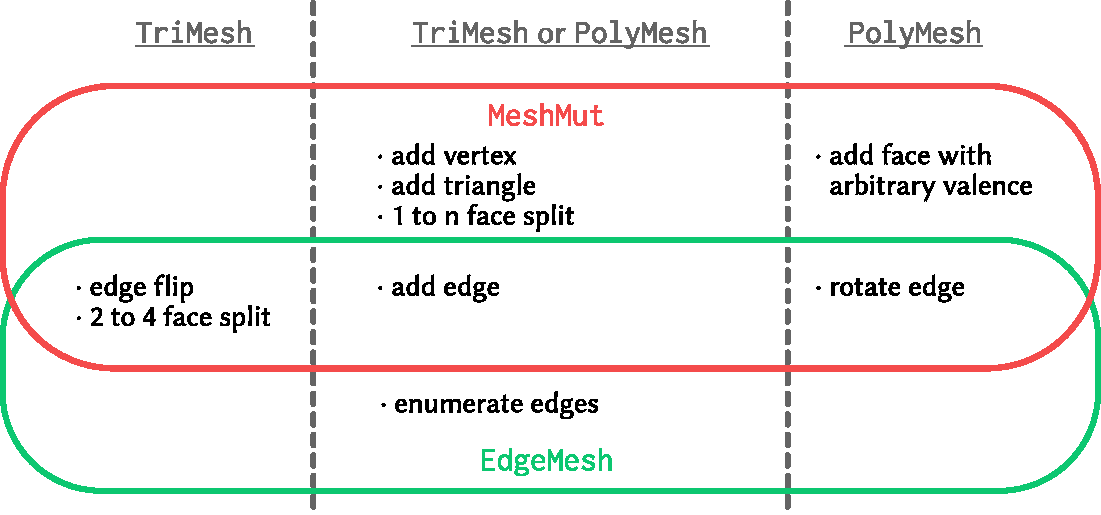
\includegraphics[width=.98\textwidth]{svg2pdf/mesh-features}
  \caption{
    A couple of example mesh features categorized by which capabilities they require (this diagram is not complete).
  }
  \label{fig:mesh-features}
\end{figure}

As already stated, basic mesh features are defined in \code{Mesh}.
There are multiple possibilities where all other features are defined:

\begin{itemize}
  \item Create a trait per combination of capabilities (e.\,g., \code{PolyMeshMut} for triangular meshes that can be mutated) and put each feature in the fitting trait.
  This works, but creates a large number of traits.
  Users might prefer to have functionality in as few traits as possible.
  \item Create a trait per single optional capability and put features only requiring one capability in the corresponding trait.
  Features requiring multiple capabilities are defined in the trait of one of those capabilities, defining all other capabilities by adding trait bounds to \code{Self}.
  For example, the method to add arbitrary faces could be defined in \code{MeshMut} with the following signature:

  \begin{rustcode}
    fn add_face(&mut self, vertices: &[VertexHandle]) -> FaceHandle
    where
        Self: PolyMesh;
  \end{rustcode}

  \item Like the last version, but put all methods into \code{Mesh}, completely declaring the required capabilities via bounds on \code{Self}.
  \item Some combination of the three explained possibilities.
\end{itemize}

None of these solutions is clearly better than the others which is part of the reason the design of the mesh traits is not finished yet.
The current solution is to define all methods in either \code{Mesh} or \code{MeshMut}.
Traits \code{EdgeMesh}, \code{TriMesh} and \code{PolyMesh} are added, but just serve as markers.
Methods requiring additional capabilities declare that via bounds on \code{Self}.
This design avoids having a large number of traits and all functionality is found in only two traits, making it easy to discover for users.
Also see figure~\ref{fig:mesh-traits}.

\subsubsection*{Mutually exclusive traits}

Special attention has to be paid to the design of \code{TriMesh} and \code{PolyMesh}.
Simply adding two traits would be incorrect, because types could implement neither or both of these traits which should be prohibited.
To solve this problem, the trait \code{Mesh} could declare an \emph{associated constant} and the two traits could be defined in terms of this constant:

\begin{rustcode}
  enum FaceKind { Triangle, Polygon }

  trait Mesh {
      const FACE_KIND: FaceKind;
  }

  trait TriMesh: Mesh<FACE_KIND = FaceKind::Triangle> {}
  trait PolyMesh: Mesh<FACE_KIND = FaceKind::Polygon> {}

  // Blanket implementation to automatically implement traits for all types
  // that also implement Mesh with the correct face kind.
  impl<T: Mesh<FACE_KIND = FaceKind::Triangle> TriMesh for T {}
  impl<T: Mesh<FACE_KIND = FaceKind::Polygon> PolyMesh for T {}
\end{rustcode}

Implementors need to define a value for the constant when implementing the trait.
\code{TriMesh} and \code{PolyMesh} are automatically implemented for these types implementing \code{Mesh} with the corresponding value.
The only problem with this approach is that it does not compile yet:
the Rust compiler still lacks the ability to check value equality within trait bounds.
Luckily, this problem can simply be worked around by using types instead of values and using an associated type instead of an associated constant.

\begin{rustcode}
  // Two types instead of two values.
  enum TriFace {}
  enum PolyFace {}

  // A trait which is only implemented for these types (not strictly
  // necessary, but avoids misuse of the API).
  trait FaceKind {}
  impl FaceKind for TriFace {}
  impl FaceKind for PolyFace {}

  trait Mesh {
      type FaceKind: FaceKind;  // Type instead of constant
  }

  trait TriMesh: Mesh<FaceKind = TriFace> {}
  trait PolyMesh: Mesh<FaceKind = PolyFace> {}

  // Blanket implementation to automatically implement traits for all types
  // that also implement Mesh with the correct face kind.
  impl<T: Mesh<FaceKind = TriFace> TriMesh for T {}
  impl<T: Mesh<FaceKind = PolyFace> PolyMesh for T {}
\end{rustcode}


\subsubsection*{Adjacency Traits}

All functionality regarding adjacency information has to be defined in traits as well.
As before, defining too many traits (e.\,g., one trait per basic adjacency query) would make the whole API more confusing while a single trait would not be flexible enough.
The current design consists of three traits (cf. figure~\ref{fig:mesh-traits}):

\begin{itemize}
  \item \textbf{\codebox{BasicAdj}}: this trait only defines \adj{F}{V} adjacency.
  This is arguably the most used neighborhood query as it is needed for basic rendering and IO.
  The trait is implemented by all mesh data structures within \code{lox}.
  \item \textbf{\codebox{FullAdj}}: requires \code{BasicAdj} and adds \adj{F}{F}, \adj{V}{F} and \adj{V}{V} queries, meaning that all queries between faces and vertices are supported.
  It is implemented by all data structures except for \code{SharedVertexMesh}.
  \item \textbf{\codebox{EdgeAdj}}: requires \code{FullAdj} and adds \adj{E}{F}, \adj{E}{V}, \adj{F}{E} and \adj{V}{E}.
  This is currently only implemented by \code{HalfEdgeMesh}.
\end{itemize}

This solution works fairly well for mesh data structures defined within \code{lox}, but has not been evaluated for potential external data structures:
The main advantage is the low number of traits which simplifies the API.
But as mentioned above, this design is likely to change in the future.

\begin{figure}[th]
  \centering
  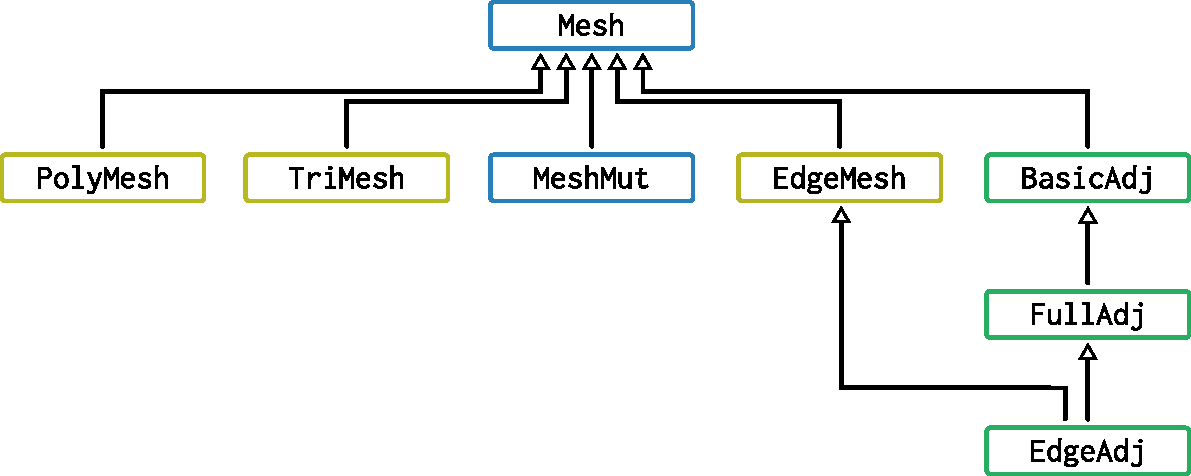
\includegraphics[width=.98\textwidth]{svg2pdf/mesh-traits}
  \caption{
    Traits currently used in \codebox{lox} to abstract over meshes.
    The arrows represent \emph{super trait bounds}, i.\,e., \codebox{Mesh} is a super trait of \codebox{MeshMut}.
    Green boxes contain traits that deal with adjacency information, yellow boxes indicate marker traits without own methods.
  }
  \label{fig:mesh-traits}
\end{figure}


\vfill
\subsubsection*{Data Structures in \codebox{lox}}

At the time of this writing, \code{lox} provides three data structures:
the shared vertex mesh, the half edge mesh and the directed edge mesh.
However, it is planned to add more data structures to the library in the near future.

%TODO: maybe actually implement this?
The half edge mesh and directed edge mesh can be configured at compile time.
Both meshes allow specifying which optional fields (e.\,g., \code{prev}) are stored and the half edge mesh offers an option to restrict the mesh to triangular faces (which does not change the underlying data structure, but makes some operations faster).
The configuration is done via a type parameter and a trait \code{Config}.
The system for the half edge mesh looks like this:

\begin{rustcode}
trait Config {
    type FaceKind: FaceKind;
    type StorePrev: Bool;
}

struct HalfEdgeMesh<C: Config> { /* ... */ }

// Type-level bool
trait Bool {}
enum True {}
enum False {}
impl Bool for True {}
impl Bool for False {}
\end{rustcode}

As mentioned previously, Rust does not yet support using constants in trait bounds.
For that reason, the \code{Config} trait uses associated types instead of associated constants to store type-level values.
The \emph{FaceKind} trait is the one defined earlier in this section.

\newpage
The following table shows which traits are implemented by which data structure.

\begin{center}
  \renewcommand{\arraystretch}{1.2}
  \setlength{\dashlinedash}{.4mm}
  \setlength{\dashlinegap}{1mm}
  \begin{tabular}{l|c:c:c}
  & \code{SharedVertexMesh} & \code{DirectedEdgeMesh} & \code{HalfEdgeMesh} \\\hline
  \code{Mesh}
    & \textcolor{flat-green-light}{\textbf{\textsf Yes}}
    & \textcolor{flat-green-light}{\textbf{\textsf Yes}}
    & \textcolor{flat-green-light}{\textbf{\textsf Yes}} \\\hdashline[.4mm/1mm]
  \code{MeshMut}
    & \textcolor{flat-green-light}{\textbf{\textsf Yes}}
    & \textcolor{flat-green-light}{\textbf{\textsf Yes}}
    & \textcolor{flat-green-light}{\textbf{\textsf Yes}} \\\hdashline[.4mm/1mm]
  \code{EdgeMesh}
    & \textcolor{red}{\textbf{\textsf No}}
    & \textcolor{red}{\textbf{\textsf No}}
    & \textcolor{flat-green-light}{\textbf{\textsf Yes}} \\\hline
  \code{BasicAdj}
    & \textcolor{flat-green-light}{\textbf{\textsf Yes}}
    & \textcolor{flat-green-light}{\textbf{\textsf Yes}}
    & \textcolor{flat-green-light}{\textbf{\textsf Yes}} \\\hdashline[.4mm/1mm]
  \code{FullAdj}
    & \textcolor{red}{\textbf{\textsf No}}
    & \textcolor{flat-green-light}{\textbf{\textsf Yes}}
    & \textcolor{flat-green-light}{\textbf{\textsf Yes}} \\\hdashline[.4mm/1mm]
  \code{EdgeAdj}
    & \textcolor{red}{\textbf{\textsf No}}
    & \textcolor{red}{\textbf{\textsf No}}
    & \textcolor{flat-green-light}{\textbf{\textsf Yes}} \\\hline
  Face kind
    & \code{TriMesh}
    & \code{TriMesh}
    & \emph{configurable}
  \end{tabular}
  \renewcommand{\arraystretch}{1.0}
\end{center}

Each data structure is tested rigorously by a number of unit tests.
Fortunately, due to the mesh abstractions, the test suite needs to be defined only once and can then be used for each data structure.
Configurable data structures are tested for multiple different configurations.
With these unit tests, new data structure implementations can be added by using \emph{test driven development}.

The unit tests construct different mesh topologies, execute various operations on them and test almost all observable properties at every step.
To avoid repetitive code, Rust macros and helper functions are used extensively, making test definitions very concise.
The test suite definition can be found in \code{src/ds/tests.rs}.


\newpage
\section{Input/Output Module}

Reading and writing meshes from/to files is a feature required by most programmers using a geometry processing library.
The library \code{lox} also offers various functionality for \enquote{IO} (input/output), including file operations.
Most of it is defined in the module \code{lox::io}.

Before implementing the functionality, the following goals were set:

\begin{itemize}
  \item \textbf{Speed}: loading and writing even large meshes should not keep the user waiting.
  \item \textbf{Convenience}: most of the time, programmers do not care about the specifics of IO and should thus be able to use most of the IO functionality very easily.
  \item \textbf{Flexibility}: somewhat contrasting the previous goal, the IO module should be flexible enough so that it can be used in virtually all situations.
  In particular, users should be able to tweak details of IO operations.
  And even if users need to load very abnormal meshes, they should never be required to write their own parser for a specific file format but be able to use the functionality of \code{lox}.
  \item \textbf{More than files}: the IO functionality should not be restricted to files.
  For example, there are sources of mesh data other than files.
  Everything that can provide or receive mesh data should be able to use the IO interface like a file.
  \item \textbf{Correct and robust}: invalid input should never crash the library.
  Instead, an error indicating the problem should be emitted.
  Additionally, reader and writers of file formats should stick to the specification as closely as possible.
  \item \textbf{Compile time correctness}: unless this conflicts with the other goals, as many programmer errors as possible should be caught at compile time.
\end{itemize}

\vfill
At the core of the IO module, a set of traits is required to abstract over all types that can provide or receive mesh data (including files).
In \code{lox}'s design, everything that can provide mesh data is called a \emph{source}, everything that can receive it is called a \emph{sink}.
The exact design of these traits is of uppermost importance for meeting the goals defined above.

An early important realization is that there are two kinds of sources and sinks each: those which can provide/receive data in any order and those who are restricted to a particular order of data.
For example, files are restricted to the specific order defined by their file format which can differ between different formats, e.\,g. \textsc{Ply} and \textsc{Obj}.
Those files have to be read/written from front to back and usually do not allow random access.
Similarly, meshes defined algorithmically provide the mesh data in the order that the algorithm creates it.
On the other hand, in-memory mesh data structures and property maps allow arbitrary access to their data.

This important distinction is reflected in the trait system by exposing \code{MemSource} and \code{MemSink} (allowing random access) as well as \code{StreamSource} and \code{StreamSink} (restricted to one order).
These traits are also shown in figure~\ref{fig:io-traits}.
This system has some similarities to the \code{Reader}/\code{Writer} and \code{Importer}/\code{Exporter} system of OpenMesh.

\begin{figure}[t]
  \centering
  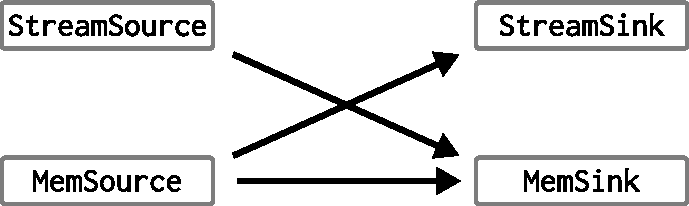
\includegraphics[width=.6\textwidth]{svg2pdf/io-traits}
  \caption{
    The core IO traits of \codebox{lox}.
    To transfer mesh data, the source or the sink (or both) has to provide random access to the
    data.
  }
  \label{fig:io-traits}
\end{figure}

\newpage

Since the \code{Stream*} versions of these traits are restricted ones, they have to define the main procedure as this specifies the order of mesh data.
This results in fairly minimal trait interfaces for those two traits:

\begin{rustcode}
  pub trait StreamSource {
      fn transfer_to<SinkT: MemSink>(self, sink: &mut SinkT) -> Result<(), Error>;
  }

  pub trait StreamSink {
      fn transfer_from<SrcT: MemSource>(self, src: &SrcT) -> Result<(), Error>;
  }
\end{rustcode}

The \code{Mem*} variants of those traits have a significantly larger interface.
\code{MemSource} contains a method to return a reference to the \enquote{core mesh} (containing the connectivity) which is required to at least implement the traits \code{Mesh} and \code{BasicAdj}.
The trait also contains methods for every predefined mesh property, a list that currently includes vertex positions, vertex normals, vertex colors, face normals and face colors.
The \code{MemSink} has a similar interface that allows adding connectivity and property data.

A difficult part of the design was to allow for different types of mesh properties.
This is required because different file formats store mesh properties with different types and some file formats even allow storing multiple types (e.\,g. \textsc{Ply}).
For example, \code{lox} should be able to read and write \code{f32} \emph{and} \code{f64} vertex positions;
reading and writing color data should work with \code{f32} \emph{and} \code{u8} channels -- with or without alpha channel.
This flexibility was achieved by making all property methods of the \code{Mem*} traits generic and providing a separate method to ask for the preferred data type.
This made the interface notably more complex, but this was accepted in order to provide a fast and flexible core interface.
Ideally, most users do not need to interact with these core traits directly anyway, making the complexity increase less of an issue.

As the core data structures (e.\,g. \code{HalfEdgeMesh}) cannot store mesh properties, external property maps are needed for those.
The user is then supposed to create a struct type that contains the core mesh and all required property meshes.
These types are called \enquote{fat meshes} in the context of \code{lox}.
In order to read mesh data from a file into a fat mesh or to write a fat mesh to a file, the fat mesh type needs to implement \code{MemSource} and \code{MemSink}.
However, implementing those traits is not trivial and requires a lot of boilerplate code.
Requiring the user to write those implementations would make using the library a lot less convenient.

Two features are offered to solve this problem.
First, \code{lox} implements and exposes a small number of predefined fat meshes in the module \code{lox::fat}.
For example, \code{fat::MiniMesh} stores the core mesh and \code{f32} vertex positions.
But more importantly, \code{lox} provides a \emph{custom derive} for both \code{Mem*} traits which allows to implement the traits by simply annotating the struct definition.
Example:

\begin{rustcode}
#[derive(MemSource, MemSink)]
struct MyMesh {
    #[lox(core_mesh)]
    mesh: HalfEdgeMesh,

    #[lox(vertex_position)]
    positions: VecMap<VertexHandle, Point3<f32>>,
}
\end{rustcode}

These \emph{custom derives} are implemented as \emph{procedural macros}: functions that operate on the source code and emit new source code.
Unfortunately, completely explaining procedural macros in this chapter is not possible.
In short, a function defined by \code{lox} receives the definition of the struct \code{MyMesh} in form of a token stream, parses it into an abstract syntax tree, inspects it and generates new Rust code in form of a token stream containing an \code|impl Mem* for MyMesh { ... }| block.
This function is called by the compiler during compilation and the generated code is then fed back into the compilation process.
This has the effect, that the \code{Mem*} traits are implemented for \code{MyMesh} without the user having to write any boilerplate code.

Another important part of the IO functionality is \emph{type casting}.
In a fat mesh, the types of mesh properties are usually fixed, e.\,g. \code{Point3<f32>} vertex positions or \code{[u8; 3]} colors.
As files may contain or require properties with a different type, the IO code should be able to deal with that type mismatch.
One possibility is to always convert between the types automatically.
While this makes the interface more convenient to use (as the problem is not exposed), it could exhibit behavior unexpected by the user.
Casting between different numeric types often requires clamping or rounding (cf. figure~\ref{fig:casting}), something the user might want to prevent or at least know about.

As with the order of data, the type of properties is ultimately determined by the \code{Stream*} sinks and sources, meaning that the responsibility for type casting lies with the \code{Mem*} part.
Those can either cast to the destination type or raise an error if they cannot handle that specific type conversion.
To make this choice easily available to the user, the custom derives support annotating one of five \emph{casting modes}: \code{none}, \code{lossless}, \code{clamping}, \code{rounding} and \code{lossy} -- the last one is the default and allows casts involving both, clamping and rounding.
A simple example:

\begin{rustcode}
#[lox(vertex_normal, cast = "lossless")]
vertex_normals: VecMap<VertexHandle, Vector3<f32>>,
\end{rustcode}

\newpage

\begin{figure}[t]
  \centering
  \setlength{\dashlinedash}{.3mm}
  \setlength{\dashlinegap}{.6mm}
  \setlength{\tabcolsep}{0mm}

  \newcommand{\lossless}{\raisebox{-.5mm}{\tikz[scale=0.15]{\fill[flat-green-light] (0,0) circle(1);}}}
  \newcommand{\clamping}{\raisebox{-.5mm}{\tikz[scale=0.15]{\fill[flat-red-light] (0,0) circle(1);}}}
  \newcommand{\rounding}{\raisebox{-.5mm}{\tikz[scale=0.15]{\fill[flat-gray-dark] (0,0) circle(1);}}}
  \newcommand{\lossy}{%
    \raisebox{-1mm}{%
      \tikz[rotate=45, scale=0.15]{%
        \begin{scope}%
          \clip (-1,0) rectangle (1,1);%
          \fill[flat-red-light] (0,0) circle(1);%
        \end{scope}%
        \begin{scope}%
          \clip (-1,0) rectangle (1,-1);%
          \fill[flat-gray-dark] (0,0) circle(1);%
        \end{scope}%
      }%
    }
  }

  \renewcommand{\arraystretch}{0.91}
  \begin{tabular}{|c|C{9mm}:C{9mm}:C{9mm}:C{9mm}:C{9mm}|C{9mm}:C{9mm}:C{9mm}:C{9mm}:C{9mm}|C{9mm}:C{9mm}|}\hline
    \hfill \textbf{$\lcurvearrowne$} \hspace{0mm}
      & \textbf{\codebox{u8}} & \textbf{\codebox{u16}} & \textbf{\codebox{u32}}
      & \textbf{\codebox{u64}} & \textbf{\codebox{u128}}
      & \textbf{\codebox{i8}} & \textbf{\codebox{i16}} & \textbf{\codebox{i32}}
      & \textbf{\codebox{i64}} & \textbf{\codebox{i128}}
      & \textbf{\codebox{f32}} & \textbf{\codebox{f64}}\\\hline

      \textbf{\codebox{u8}}
        & \lossless & \lossless & \lossless & \lossless & \lossless
        & \clamping & \lossless & \lossless & \lossless & \lossless
        & \lossless & \lossless \\\hdashline
      \textbf{\codebox{u16}}
        & \clamping & \lossless & \lossless & \lossless & \lossless
        & \clamping & \clamping & \lossless & \lossless & \lossless
        & \lossless & \lossless \\\hdashline
      \textbf{\codebox{u32}}
        & \clamping & \clamping & \lossless & \lossless & \lossless
        & \clamping & \clamping & \clamping & \lossless & \lossless
        & \rounding & \lossless \\\hdashline
      \textbf{\codebox{u64}}
        & \clamping & \clamping & \clamping & \lossless & \lossless
        & \clamping & \clamping & \clamping & \clamping & \lossless
        & \rounding & \rounding \\\hdashline
      \textbf{\codebox{u128}}
        & \clamping & \clamping & \clamping & \clamping & \lossless
        & \clamping & \clamping & \clamping & \clamping & \clamping
        & \rounding & \rounding \\\hline
      \textbf{\codebox{i8}}
        & \clamping & \clamping & \clamping & \clamping & \clamping
        & \lossless & \lossless & \lossless & \lossless & \lossless
        & \lossless & \lossless \\\hdashline
      \textbf{\codebox{i16}}
        & \clamping & \clamping & \clamping & \clamping & \clamping
        & \clamping & \lossless & \lossless & \lossless & \lossless
        & \lossless & \lossless \\\hdashline
      \textbf{\codebox{i32}}
        & \clamping & \clamping & \clamping & \clamping & \clamping
        & \clamping & \clamping & \lossless & \lossless & \lossless
        & \rounding & \lossless \\\hdashline
      \textbf{\codebox{i64}}
        & \clamping & \clamping & \clamping & \clamping & \clamping
        & \clamping & \clamping & \clamping & \lossless & \lossless
        & \rounding & \rounding \\\hdashline
      \textbf{\codebox{i128}}
        & \clamping & \clamping & \clamping & \clamping & \clamping
        & \clamping & \clamping & \clamping & \clamping & \lossless
        & \rounding & \rounding \\\hline
      \textbf{\codebox{f32}}
        & \lossy & \lossy & \lossy & \lossy & \lossy
        & \lossy & \lossy & \lossy & \lossy & \rounding
        & \lossless & \lossless \\\hdashline
      \textbf{\codebox{f64}}
        & \lossy & \lossy & \lossy & \lossy & \lossy
        & \lossy & \lossy & \lossy & \lossy & \lossy
        & \lossy & \lossless \\\hline
  \end{tabular}
  \renewcommand{\arraystretch}{1.0}
  \caption{
    Casts between numerical types.
    For some conversion, some values might need to be clamped\,\protect\clamping{}, rounded\,\protect\rounding{} or both\,\protect\lossy to be representable in the target type.
    If all values of the source type can exactly be represented in the target type, it is marked with \protect\lossless{}.
  }
  \label{fig:casting}
\end{figure}

For each file format, \code{lox} defines a \code{Reader} and \code{Writer} which implement \code{StreamSource} and \code{StreamSink}, respectively.
The four sink/source traits constitute the mid-level IO interface: it is already abstracted, but still not particularly easy to use.
As low-level interface, each \code{Reader} and \code{Writer} exposes format-specific methods which allow reading data of that format without the source/sink interface.
To provide a convenient high-level interface, too, a couple of functions are directly exported by the IO module, including the following ones (here slightly simplified):

\begin{rustcode}
fn read_file<SinkT: Empty + MemSink>(path: &Path)
    -> Result<SinkT, Error>
{ … }

fn write_file<SrcT: MemSource>(path: &Path, src: &SrcT)
    -> Result<(), Error>
{ … }
\end{rustcode}

This allows users to write \code{let mesh: MyMesh = io::load_file("foo.ply");}, for example.
That code automatically detects the correct file format, instantiates the corresponding \code{Reader}, uses the source/sink traits to transfer mesh data and returns the new instance of \code{MyMesh}.

\vspace{1.5cm}

Currently, \code{lox} has full support for the \textsc{Ply} and \textsc{Stl} file formats, with more file formats (including \textsc{Obj}) planned for the near future.
To guarantee a high implementation quality and adherence to the (unfortunately often very imprecise) format's specifications, different tests are used.
For one, a number of unit tests read and write various meshes with various properties and check if the written file or the read mesh is correct.

Furthermore, so called \emph{fuzzing} tests are used.
In those, a \emph{fuzzer} automatically generates a large number of inputs that are given to the parsers of the different file formats.
The inputs are not completely random, however.
Instead, the fuzzer tries to achieve a high code coverage by analyzing which statements and branches are executed for what inputs and then tries to systematically generate inputs to reach previously unreached code.
That way, advanced fuzzers can generate valid input files from just analyzing and trying to optimize code coverage (cf. \cite{jpegfuzzing}).

The goal of fuzzing tests is usually to find crashes and other unexpected behavior.
This is particularly useful for parsers, as they often have to deal with many obscure edges cases.
Due to fuzzing tests, a couple of bugs were found and fixed in \code{lox}'s parsers.



\vspace{1.5cm}


With this core system of traits and the three different layers of convenience/abstraction, all initial goals are met for the most part.
There are still a number of possible improvements, but the system as offered is already fairly fast, flexible and convenient to use.
\vspace{6mm}


\newpage
\section{Performance Optimizations}

As execution speed is an important goal of \code{lox}, several critical parts of the library were analyzed and optimized to improve performance.
This chapter gives an overview of some of the optimization work that went into this library.

Writing idiomatic Rust code usually already makes sure that the compiled code performs reasonably well, meaning that correctness can be the programmer's main focus when initially writing the code.
To improve speed further, several approaches were used.
For one, a couple of benchmarks comparing \code{lox} to OpenMesh in different situations were created and executed regularly, providing a good baseline.
The programs \emph{perf}\footnote{Performance analyzer for Linux} and Intel$^\text{\tiny ®}$~VTune$^\text{\tiny ™}$~Amplifier\footnote{Website: \url{https://software.intel.com/en-us/vtune}} were used for profiling, i.\,e., to gather different information about a program's runtime behavior.
To inspect generated machine code, the tools Cutter\footnote{Website: \url{https://github.com/radareorg/cutter}} and Godbolt Compiler Explorer\footnote{Website: \url{https://godbolt.org/}} were used.

By profiling different workloads and inspecting the machine code, many performance problems and hotspots were identified across the code base.
Generally, those problems were fixed by rewriting small parts of the code or providing hints to the compiler.
In some cases, the optimizer did not inline tiny functions.
This could be fixed by adding the \code{#[inline(always)]} attribute to those functions, often resulting in a measurable increase in performance.
Important functions that are called very rarely (e.\,g., functions constructing an error object) are instead annotated with \code{#[inline(never)]} and \code{#[cold]}, improving code generation for callers of these functions.

Before any code was changed, at least one benchmark executing that part of the code was written.
That way, the performance impact of a change could always be measured directly.
Changes that would not result in a measurable improvement (or even in decreased performance) would be reverted.

\vspace{-1mm}
\subsubsection*{IO Optimizations}

Most IO operations can fail for several reasons: the operating system might raise an error when interacting with the file system, the parser could detect a malformed input file, sinks or sources can raise errors about incompatible types, and more.
As a consequence, many functions in \code{lox::io} return \code{Result<_, Error>} where \code{Error} is the error type defined in the IO module.
This error type was an enum listing all potential error cases, with some variants storing several fields to describe the error.
Over time, the size of this type grew to 56 bytes.

This is a problem as the return type of many functions would have a significant size, increasing the size of many stack frames.
Functions that were not inlined required a fairly long function prologue and epilogue to prepare this stack data.
To solve this problem, \code{Error} was renamed to \code{ErrorKind} and a new type \code{Error} was defined with a single field of type \code{Box<ErrorKind>}.
In short: the actual error data is now heap allocated and \code{Error} itself is only 8 bytes large.
Additionally, due to null pointer optimization, \code{Result<(), Error>} (often used as return type) is also only 8 bytes in size, meaning it can be returned from functions in a single CPU register, further improving speed.
This layout change resulted in performance improvements for most IO operations between 10\% and 30\%.

Reading \textsc{Ply} files proved particularly challenging as the format supports dynamic lists and a dynamic type system with ten numeric types.
The header of a \textsc{Ply} file defines a list of elements, each defining a list of properties which in turn can either be a list or a scalar.
List elements and scalar values can be one of ten numeric types.
The list property's length is not specified in the header, can vary with each element and is stored next to the list data.
This is problematic as the reader needs to read one property at a time instead of being able to consume a lot of data at once.
Additionally, to read the correct number of bytes for a property, the property's type has to be checked, introducing many branches into the hot inner loop.

To somewhat circumvent the problem, a function pointer was prepared for each property and element.
While this introduces a number of dynamic calls in the hot loop, a lot of checks can be done before reading body data, overall improving reading performance.
The best solution would probably be to parse the file header and then generate specialized machine code for reading body data.
While this could probably improve performance by a large factor, this solution was considered too elaborate for this thesis.


\vspace{-1mm}
\subsubsection*{Data Structure Optimizations}

The main micro-optimization improving performance of data structure operations was related to bound checking.
To guarantee memory safety, Rust performs bound checks whenever array-like structures are indexed.
These checks can usually be removed by the optimizer and therefore are not a big problem.
However, in the context of \code{lox}'s data structures, the optimizer was not able to remove bounds checks most of the time, meaning that a significant runtime overhead was caused by those checks.

Bound checks can be manually removed by using the method \code{get_unchecked}.
This function is marked as \code{unsafe}, meaning that calling it requires an \code{unsafe} block.
This was used for all internal indices, while indices passed in by the user were still checked once.
To improve robustness of this solution, Rust's strong type system was used to distinguish between indices that were proven to be valid and indices that might be invalid.
The library \code{stable-vec} -- offering the underlying dynamic array data structure -- was also optimized to remove unnecessary bound checks.
These optimizations improved overall performance by roughly 20\%.

Another important optimization is based on an additional invariant held by the half edge mesh and directed edge mesh.
Chapter~\ref{chap:background-geometry-processing} states that these data structures store one arbitrary outgoing half edge per vertex.
The implementations in \code{lox} make sure that if a vertex is a boundary vertex, the half edge stored in the \code{outgoing} field is a boundary half edge as well.
This requires only a bit more work in methods mutating the mesh, but means that checking whether a vertex lies on the boundary is a lot faster, as only one adjacent half edge has to be checked.
This optimization is also used in OpenMesh.


\newpage
\section{Overview}

The project consists of three crates: \code{lox} (the main one), \code{lox-macros} and \code{lox-cli}.
The crate \code{lox-macros} is a library crate defining the procedural macros reexported by \code{lox}.
It exists for a purely technical reason: currently, Rust requires procedural macros to be defined in their own crate.
This restriction is likely to be lifted in the future, meaning the procedural macro definitions will be moved to the crate \code{lox} and \code{lox-macros} will be removed.

Unlike the others, \code{lox-cli} is an application crate that is not part of the library \code{lox}, i.\,e., it is not included in external projects that use \code{lox}.
Instead, it exists for three different purposes: it serves as an example for how to use \code{lox}, it is used as a test for \code{lox}'s capabilities and it is supposed to become a handy helper application for everyone working with meshes.
Currently, it supports converting meshes between different files formats (the ones supported by \code{lox}) and displaying various information about a mesh file.
Both operations can be tweaked via various command line parameters.
More features will be added in the near future.

The following list shows \code{lox}'s modules, excluding very small ones.
Modules marked with~* are or will be optional modules that can be disabled via Cargo features.

\begin{itemize}
  % TODO: maybe add more algorithms if you manage to implement more
  \item \textbf{\codebox{algo}}*: will offer various different mesh algorithms.
  Currently very incomplete: only a couple of example algorithms are implemented, including the subdivision algorithm \enquote{sqrt3} \cite{kobbelt20003}, Dijkstra's algorithm \cite{dijkstra1959note} and a simple smoothing algorithm.
  \item \textbf{\codebox{cast}}: utilities for casting numerical types (see \autoref{chap:io}).
  \item \textbf{\codebox{ds}}: implementations of shared vertex mesh, half edge mesh and directed edge mesh (see \autoref{chap:mesh-traits}) plus various helper utilities.
  \item \textbf{\codebox{fat}}: fat meshes \code{MiniMesh} and \code{AnyMesh} (see \autoref{chap:io}).
  \item \textbf{\codebox{handle}}: handle types for faces, edges and vertices, the \code{Handle} trait and some utility functions (cf. \autoref{chap:memory-layout}).
  \item \textbf{\codebox{io}}*: IO traits, implementation of file formats (currently \textsc{Ply} and \textsc{Stl}) and other IO related functionality.
  \item \textbf{\codebox{map}}: property map traits and implementations (cf. \autoref{chap:memory-layout}).
  \item \textbf{\codebox{prop}}: abstractions over everything that can be treated like a 3D position (\code{Pos3Like}), a 3D vector (\code{Vec3Like}) or a color (\code{ColorLike}).
  \item \textbf{\codebox{refs}}: defines types that store a handle and a reference to the mesh, therefore representing a reference to a specific element of a mesh.
  These types expose various convenience methods which are defined in terms of methods of the mesh.
  \item \textbf{\codebox{shape}}*: will offer different shape definitions that can be used as a \code{StreamSource} to easily create meshes from abstract shape definitions.
  Currently, only UV-spheres, 2D-discs and tetrahedra are implemented.
  \item \textbf{\codebox{traits}}: defines all mesh traits (cf. \autoref{chap:mesh-traits}).
\end{itemize}

